\documentclass[addpoints]{exam}

\usepackage{graphbox}
\usepackage{hyperref}
\usepackage{listings}
\usepackage{tabularx}
\usepackage{tikz}
\usetikzlibrary{positioning}

% Header and footer.
\pagestyle{headandfoot}
\runningheadrule
\runningfootrule
\runningheader{CSCI 155}{Homework 1}{Spring 2019}
\runningfooter{}{Page \thepage\ of \numpages}{}
\firstpageheader{}{}{}

\qformat{{\large\bf \thequestion. \thequestiontitle}\hfill[\totalpoints\ points]}
\boxedpoints
% \printanswers

\title{Homework 1: 2D Graphics}
\author{CSCI 155 Computer Graphics\\Pitzer College\\Spring 2019}
\date{\numpoints\ points, Due: 5p.m. on 18 Feb}

\begin{document}
\maketitle

% This refresher provides an indication of what you are expected to know coming into this course. You may find in some of the questions below that required details are missing. If so, it is assumed that you are knowledgeable enough to make reasonable decisions based on the context and/or the provided information. You need not be on top of the math but it is expected that you have sufficient background to understand the pages that show up when you search online for help.

% The refresher is not graded and does not have to be submitted. If there is something in it that you would like to discuss, I will be happy to do so in our meeting. You are welcome to post to the forum in the meanwhile.


\begin{questions}

  \titledquestion{Geometry trumps JS}[0]

  WebGL sends data to the GPU as a {\it typed} JavaScript array, e.g. the following lines in {\tt triangle.js}.
  \begin{lstlisting}[frame=single]
    var vertices = new Float32Array([-1, -1, 0, 1, 1, -1]);
    // ...
    gl.bufferData( gl.ARRAY_BUFFER, vertices, gl.STATIC_DRAW );
  \end{lstlisting}    
  The file {\tt MV.js} in the {\tt Common} folder defines abstractions that allow programs to be written in terms of geometric entities, e.g. {\it vectors}, instead. It also defines a function to convert these abstract data types to the required JavaScript types when needed. Using these, the above code can be written as follows.
  \begin{lstlisting}[frame=single]
    var vertices = [vec2(-1, -1), vec2(0, 1), vec2(1, -1)];
    // ...
    gl.bufferData( gl.ARRAY_BUFFER, flatten(vertices), gl.STATIC_DRAW );
  \end{lstlisting}    
  This allows the program to use constructs that are more natural to the application, e.g. vectors, as opposed to catering to lower level JavaScript details. Note that {\tt MV.js} must be included in {\tt triangle.html} for this to work.

  Go over the file {\tt MV.js} in order to get familiar with the types and functionality that it offers. You need not spend too much time understanding the body of the functions, as long as you can infer, e.g. from the name, what each function does. In your code for the following problems, prefer using geometric primitives and operations from {\tt MV.js} over those provided by JavaScript.
  
  \titledquestion{Mapping and Linear Interpolation}[0]
  \label{q:interpolate}

  \begin{tabularx}{\linewidth}{cX}
    \raisebox{-\totalheight}{
      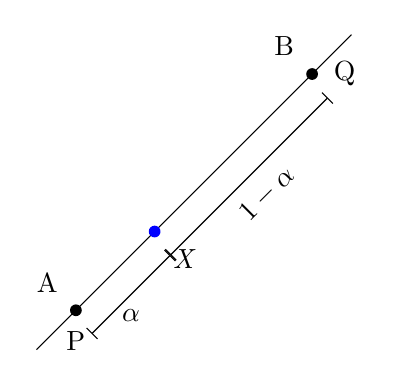
\begin{tikzpicture}
        \draw (0,0) -- (4,4);
        \node[circle,fill,inner sep=1.5pt] at (.5,.5) (P){};
        \node[circle,fill,inner sep=1.5pt] at (3.5,3.5) (Q) {};
        \node[circle,fill,blue,inner sep=1.5pt] at (1.5,1.5) (X) {};
        \node[below  = 2pt of P]{P};
        \node[right = 2pt of Q]{Q};
        \node[below right = 2pt of X]{\it X};
        \node[above left = 2pt of P]{A};
        \node[above left = 2pt of Q]{B};

        \draw[|-|] (0.7,0.2) -- node[midway,below=2pt]{$\alpha$}(1.7,1.2);
        \draw[|-|] (1.7,1.2) -- node[midway,sloped,below=2pt]{$1-\alpha$}(3.7,3.2);
      \end{tikzpicture}
    }
    &
    In the figure on the left, $X$ lies on the line segment $PQ$ such that
    \[
      |PX| : |XQ| = \alpha:(1-\alpha)\;,\; 0 \leq \alpha \leq 1,
    \]
    which leads to
    \[
      X = \alpha Q + (1-\alpha) P.
    \]
    $X$ is thus said to be an \href{https://en.wikipedia.org/wiki/Affine_combination}{\it affine combination} of $P$ and $Q$.
    
    Imagine a mapping from the range $PQ$ to a new range $AB$. Write a function {\tt map\_point} that takes $P$, $Q$, $A$, $B$, and $X$ as parameters and uses the {\tt mix} function from the file {\tt MV.js} to compute and return the mapping of $X$ to the range $AB$. This function will by used in many of the questions below.
  \end{tabularx}
  
  \titledquestion{Triangle in a Triangle in a Triangle ...}[20]
  
  \begin{figure}
    \centering
    \begin{tabular}{cc}
      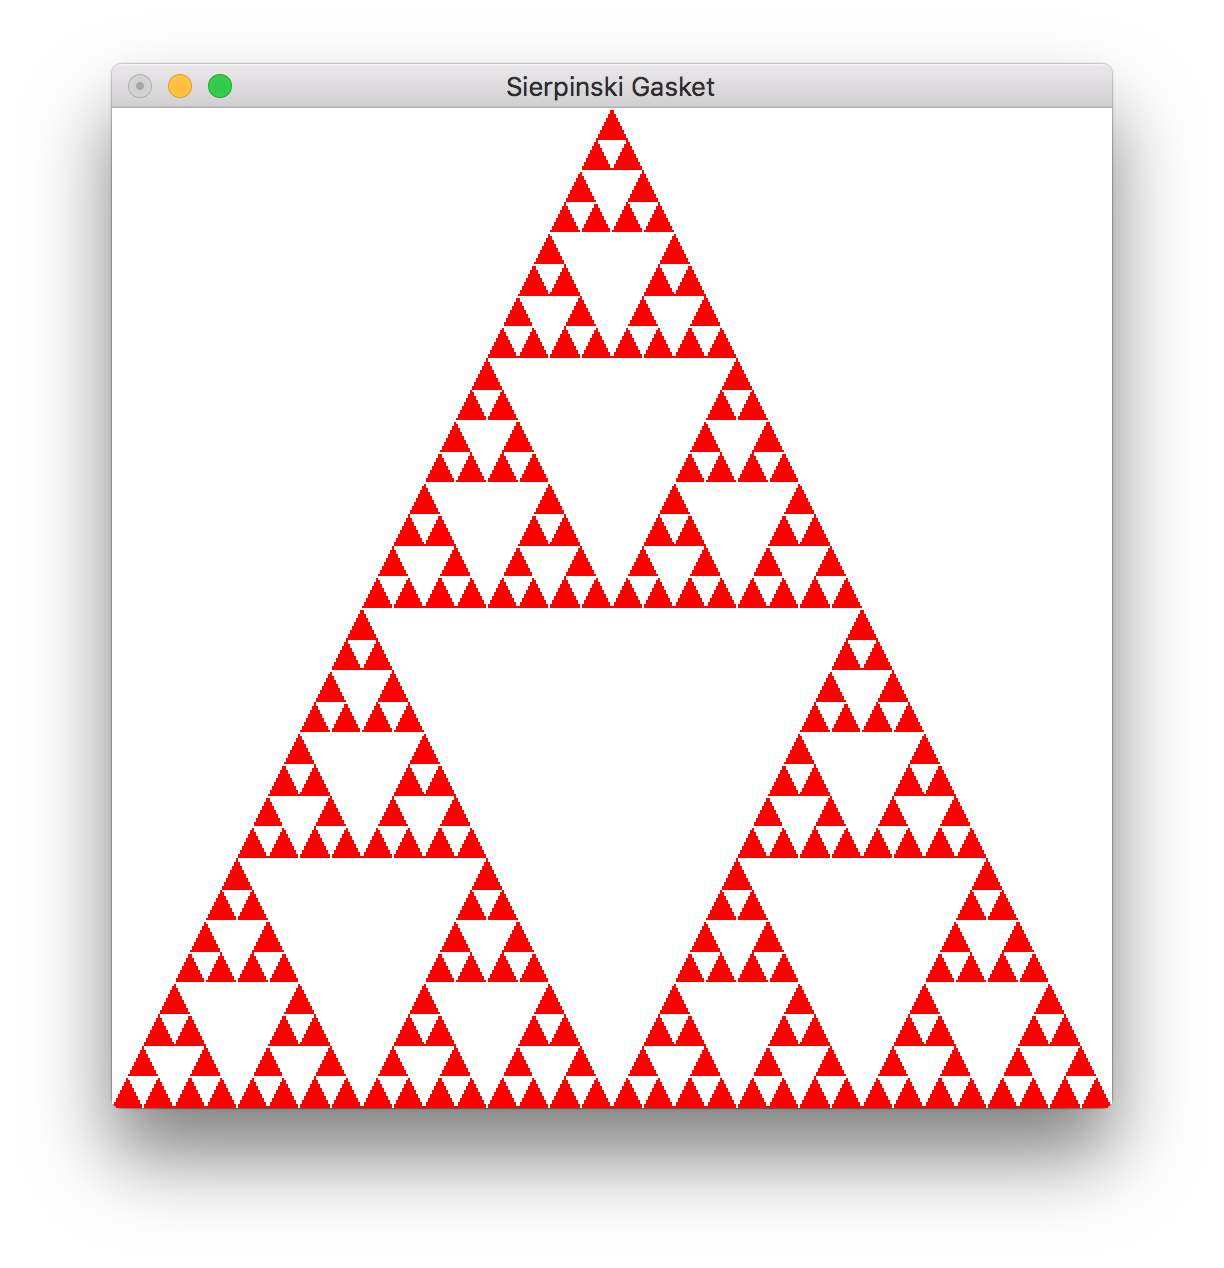
\includegraphics[width=.4\linewidth]{sierpinski}
      &
      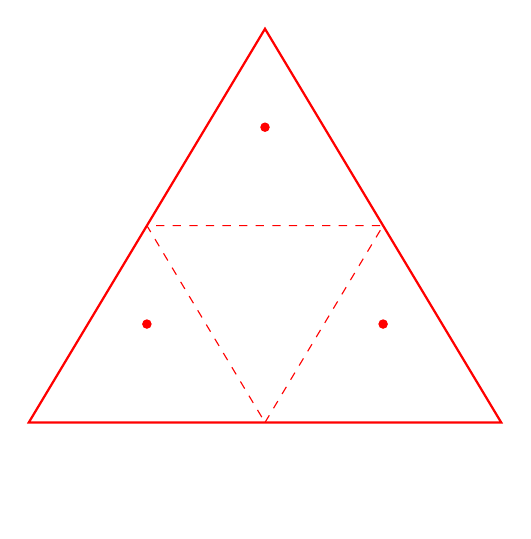
\begin{tikzpicture}
        \draw[red,thick] (0,0) -- (6,0) -- (3,5) -- cycle;
        \draw[red,dashed] (3,0) -- (4.5,2.5) -- (1.5,2.5) -- cycle;
        \draw[red,fill] (1.5, 1.25) circle (1.5pt);
        \draw[red,fill] (4.5, 1.25) circle (1.5pt);
        \draw[red,fill] (3, 3.75) circle (1.5pt);
        
        \node at (3,-1) {};
      \end{tikzpicture}\\
      (a) & (b)
    \end{tabular}
    \label{fig:sierpinski}
    \caption{(a) A Sierpinski triangle at recursion level 5. (b) The recursive step in the generation of the Sierpinski triangle.}
  \end{figure}
  
  The \href{https://en.wikipedia.org/wiki/Sierpinski_triangle}{Sierpinski triangle} is a \href{https://en.wikipedia.org/wiki/Self-similarity}{self-similar} geometric shape with many interesting properties, not the least of which is the variety of ways in which it can be generated. A sample triangle is shown in Figure \ref{fig:sierpinski}a).

  For this problem, the Sierpinski triangle is defined recursively as illustrated in Figure \ref{fig:sierpinski}b). Starting with a triangle, connect all its edge midpoints. This yields 4 new triangles. Repeat the process for all the new triangles shown with a dot in them. Do not subdivide the triangle in the middle (without a dot). Note that the dots in the figure are for demonstration purposes only--they are not part of the Sierpinski triangle.

  Write a program to generate the Sierpinski triangle at any desired recursion level.
  \underline{Files}: {sierpinski.html, sierpinski.js}
  
  \titledquestion{Approximating a Smooth Surface: $\lim\limits_{n\rightarrow\infty} \diamond = \circ$}[20]
  \begin{center}
    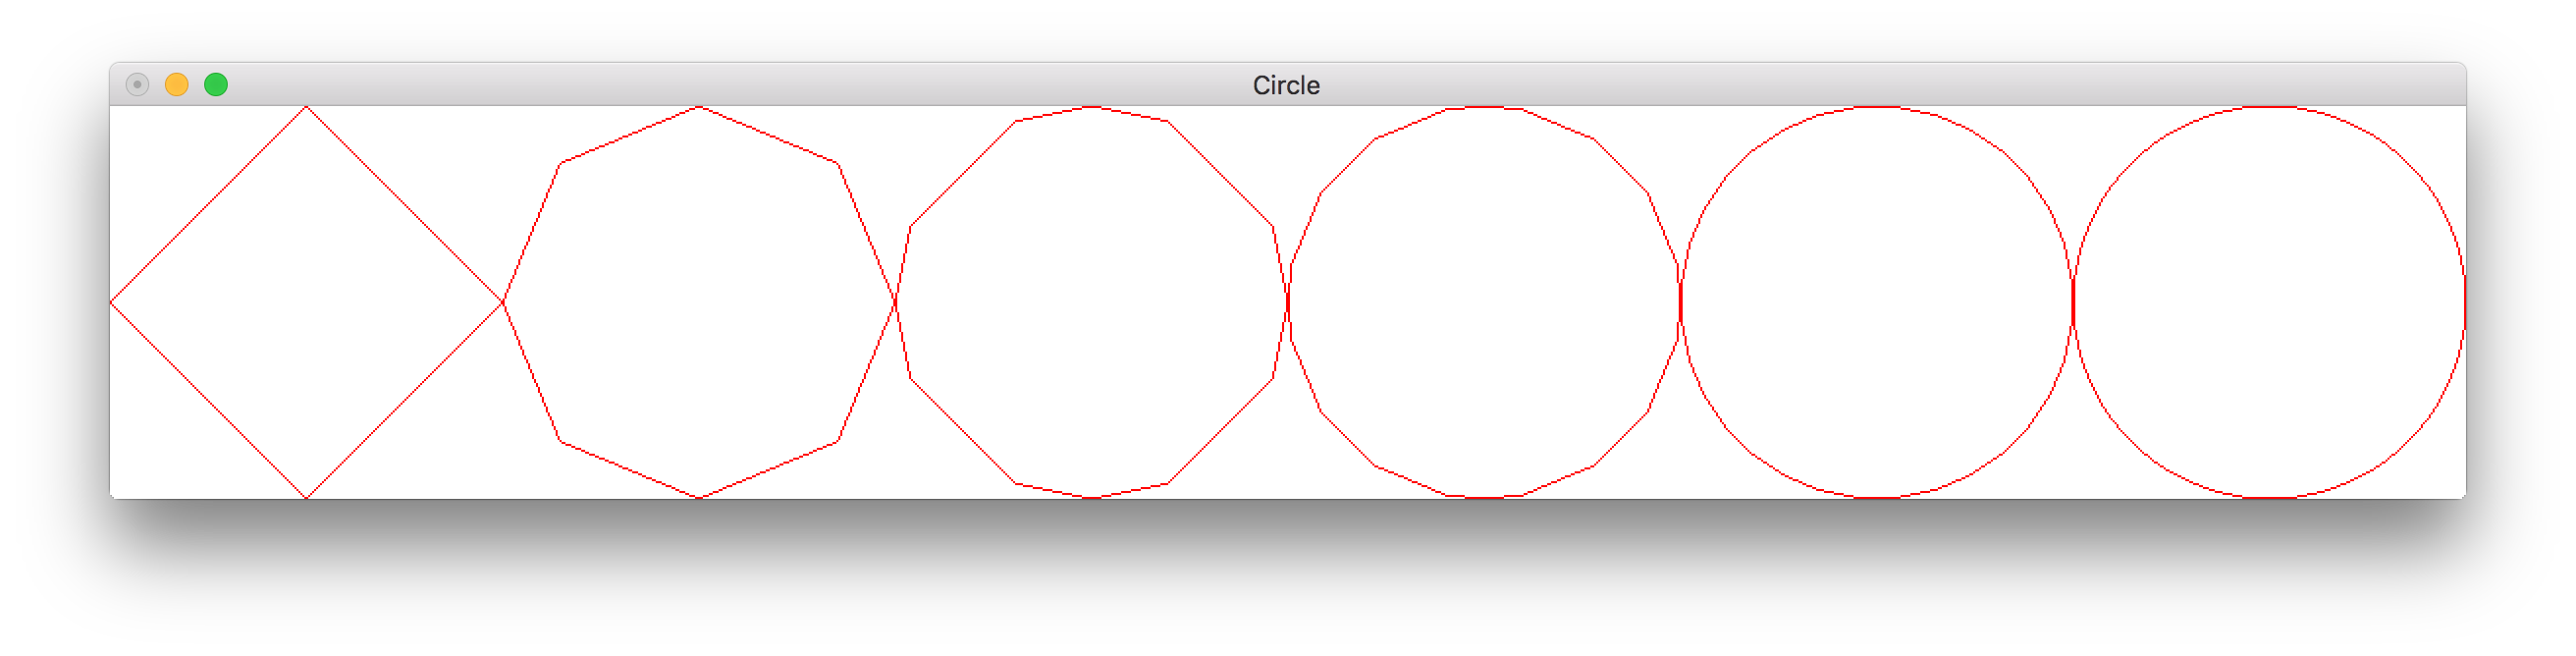
\includegraphics[width=\linewidth]{circle}
  \end{center}

  \begin{tabularx}{\linewidth}{lX}

    \raisebox{-\totalheight}{
      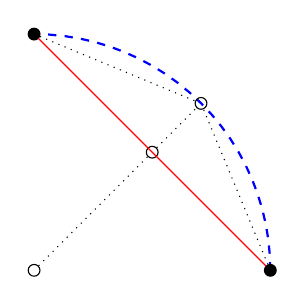
\begin{tikzpicture}
        \draw [blue,thick,dashed,domain=0:90] plot ({3*cos(\x)}, {3*sin(\x)});    
        node[circle,fill]{}(
        \node [draw,circle,fill,inner sep=1.5pt] at (0,3) (a){};
        \node [draw,circle,fill,inner sep=1.5pt] at (3,0) (b){};
        \node [draw,circle,inner sep=1.5pt] at (0,0) (c){};
        \node [draw,circle,inner sep=1.5pt] at (1.5,1.5) (p){};
        \node [draw,circle,inner sep=1.5pt] at (2.12,2.12) (q){};

        \draw [red] (a) -- (b);
        \draw [dotted] (c) -- (p);
        \draw [dotted] (p) -- (q);
        \draw [dotted] (a) -- (q);
        \draw [dotted] (b) -- (q);
      \end{tikzpicture}
    }
    &
    This problem explores the approximation of a smooth shape by a many-sided polygon. Starting from a diamond on the left in the above figure, each successive shape is recursively generated by inserting edge midpoints into the shape and projecting the new points to the circumference of the circle being approximated. This is illustrated in the figure on the left. The red line is approximating the blue arc. In the subdivision steo, the midpoint of the red line is inserted and projected to the arc. The red line is then replaced with the dotted black line.

    Generate the above figure by repetitively refining a coarse initial approximation.
  \end{tabularx}
  \underline{Files}: {circle.html, circle.js}

  \titledquestion{Maxwell's Triangle}[10]
  \label{q:maxwell}
  
  \begin{tabularx}{\linewidth}{cX}
    \raisebox{-\totalheight}{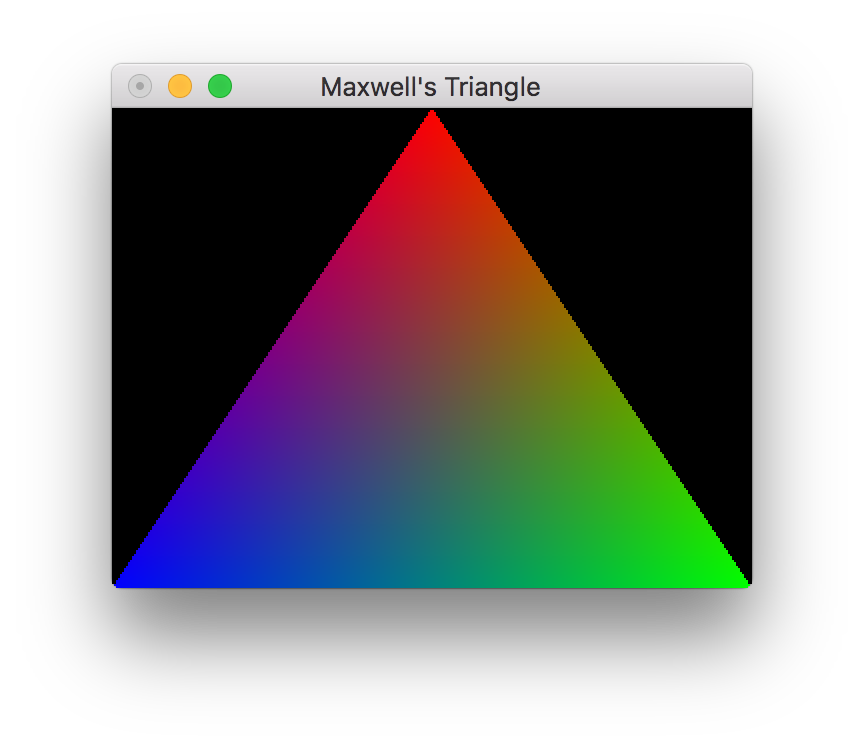
\includegraphics[width=.35\linewidth]{maxwell}}
    &
    \href{https://en.wikipedia.org/wiki/James_Clerk_Maxwell}{James Clerk Maxwell} is best known for his work in electromagnetic radiation resulting in the well known \href{https://en.wikipedia.org/wiki/Maxwell\%27s_equations}{Maxwell's equations}.
    
    Not surprisingly, he was also among the first ones to explore the \href{https://spie.org/publications/pm105_32_maxwell_triangle?SSO=1}{trichromatic theory of color}. This has led to what is now known as \href{http://www.appstate.edu/~steelekm/classes/psy3215/Maxwell.htm}{Maxwell's triangle}, simply called the \href{https://en.wikipedia.org/wiki/Color_triangle}{color triangle}. It is a triangle with the primary colors at its vertices and its interior shaded by linear combinations of the colors at the vertices. At any interior point, the amount of color contributed by a vertex is proportional to the distance of the vertex from that point.
  \end{tabularx}

    In WebGL, if the endpoints of a line segment are of different color, each point on the line segment is rendered with a color value that is interpolated from the endpoints' colors. The same applies to polygons. Use this property to display Maxwell's triangle: an equilateral triangle whose vertices are red, green, and blue.\\
  \underline{Files}: {maxwell.html, maxwell.js}
  
  \titledquestion{Color Interpolation}[20]
  \label{q:colorbar}.
  
  \begin{center}
    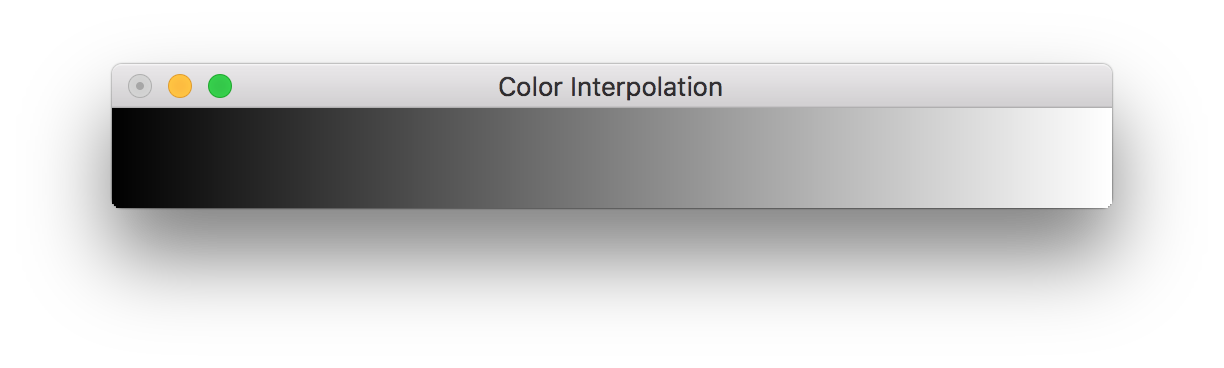
\includegraphics[width=\linewidth]{barbw}\\
    \vspace{-75pt}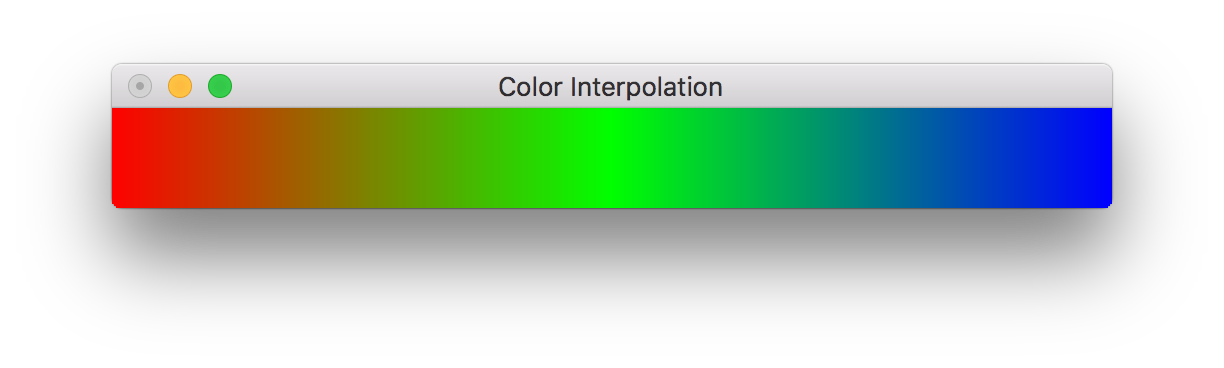
\includegraphics[width=\linewidth]{barrgb}
  \end{center}
  \vspace{-25pt}Problem \ref{q:maxwell} relied on the GPU's native color interpolation. For this problem, you will draw color bars for which you will perform the interpolation using the {\tt map\_point} function from Problem \ref{q:interpolate}.

  Display the colorbars above in your display window with the grayscale bar above the color bar. Each bar is comprised of vertical lines rendered next to each other, i.e. on adjacent pixels, in the display window. Both bars have the same dimensions. The width has to be sufficiently large to include every color in the following RGB ranges.
  \begin{itemize}
  \item (0,0,0) to (255, 255, 255), and
  \item (255,0,0) to (0, 255, 0) to (0, 0, 255).
  \end{itemize}
  \noindent\underline{Files}: {colorbar.html, colorbar.js}

  \titledquestion{The Mandelbrot Set}[30]

  The sequence $z_n$ over a complex number, $c$, is defined for positive integers, $n$, as
  \[
    z_n(c) = \left\{
      \begin{array}{l@{\quad}l}
        0 & n = 0\\
        z^2_{n-1}(c)+c & \textrm{otherwise}
      \end{array}
    \right.
  \]

  \begin{figure}
    \centering
    \begin{tabular}{cc}
      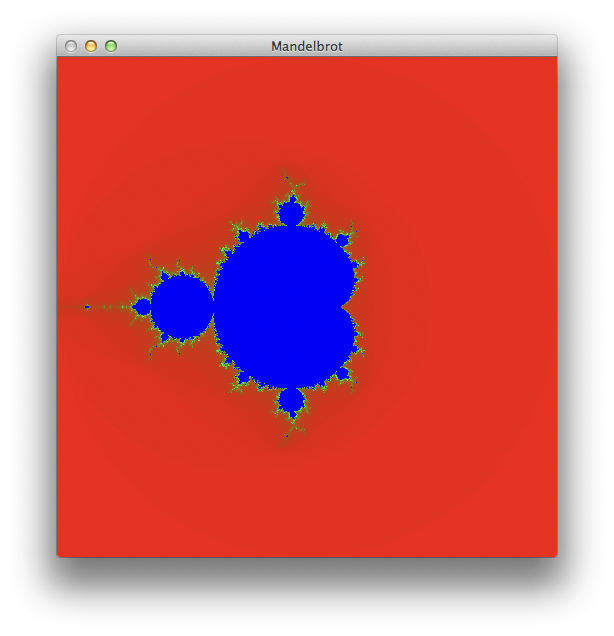
\includegraphics[width=.47\linewidth]{mandelbrot1}& 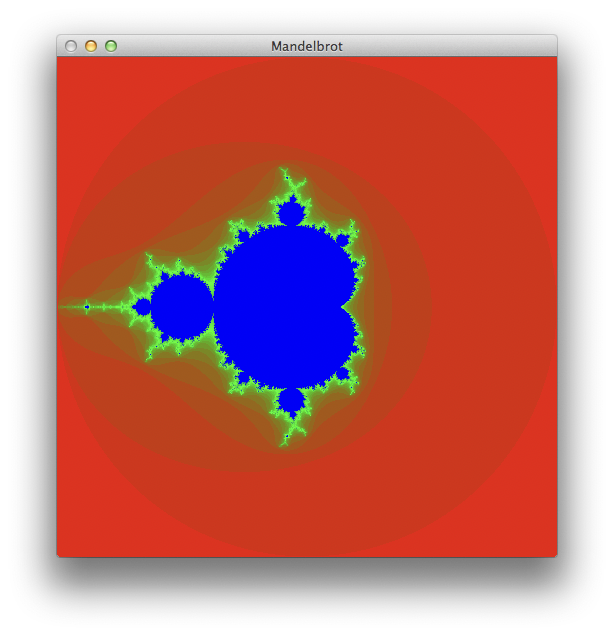
\includegraphics[width=.47\linewidth]{mandelbrot2}\\
      (a) & (b)
    \end{tabular}
    \label{fig:mandel}
    \caption{The Mandelbrot set for $n_t = 100$. Points at the corners of the windows are outside the circle of radius 2, and $z_n$ escapes for these points at $n=0$. They are thus completely red. The points in blue toward the center of the image are the ones for which $z_n$ up to $z_{100}$ has not escaped. (a) Uniform color interpolation from Red to Green to Blue. (b) Adjusted interpolation.}
  \end{figure}
  
The \href{http://en.wikipedia.org/wiki/Mandelbrot_set}{Mandelbrot set}, $M$, is the set of all complex numbers, $c$, such that $z_n$ above is bounded, i.e. $|z_n|$ is finite for all $n$. It can be shown that if for some $n = n_0$, $|z_{n_0} > 2|$, then the sequence $z_n$ {\it escapes to infinity}, i.e. $|z_n|$ is not bounded for $n > n_0$. This leads to the conclusion that $\forall c \in M\, z_n(c) \leq 2$. Note that since $z_1 = c$, the above condition also implies that $|c| \leq 2$.
The above yields the following two handy conditions whose fulfillment by a complex number, $c$, establishes its membership in $M$:
\begin{enumerate}
\item $|c|\leq 2$
\item $\forall n\geq 0\, z_n(c)\leq 2$
\end{enumerate}
The value of $n$ for which condition 2 becomes false for a given $c$ is dubbed the {\it escape time} of $c$.

Write a program to visualize the Mandelbrot set. You will need the following steps.
\begin{itemize}
\item Map $Re(c)$ and $Im(c)$ to the x and y axes respectively.
\item Your viewing rectangle should span the ranges [-2,2] in the x and y directions. The origin lies at the center of the window.
\item Map every coordinate in the viewing window to its corresponding $c$ and determine its escape time. Set an appropriately high threshold $n_t$, such that, if $z_n(c)$ has not escaped till $n = n_t$, you may assume that $c \in M$.
\item Color the pixel according to its escape time such that an escape time of 0 corresponds to red, pixels whose corresponding $c$ have not escaped are colored blue, and pixels whose $c$ has escaped between 0 and $n_t$ are colored green. This is a similar color interpolation as in Problem \ref{q:colorbar}. An example for $n_t=100$ is shown in Figure \ref{fig:mandel}a).
\item Figure \ref{fig:mandel}a). contains a lot of red. Can you figure out why? It is possible to adjust the color interpolation to yield Figure \ref{fig:mandel}b). Adjust your interpolation function to yield an aesthetically appealing coloring of your choice. Some strategies you could implement are
  \begin{itemize}
  \item move green away from the middle of the range
  \item use more colors for interpolation
  \item use non-linear interpolation
  \end{itemize}
\end{itemize}
\end{questions}

\end{document}



